\chapter{Background Literature}
\label{BackgroundLit}

\section{Introduction}
\label{BL:Intro}
This chapter reviews extant literature surrounding the design and deployment of technologies for and with people with dementia, focusing particularly on research published in the ACM Digital Library over the past 15 years. This chapter aims to answer topics centring on the research questions in regards to: participation and technology development with people with dementia; ethical complexities researchers face in everyday dementia interactions; representation of dementia; and the different stakeholders and interests that are designed for (or neglected). This chapter is split into three subsections that ultimately provide four areas of investigation that the thesis examines.


\section{Dementia and HCI}
\label{BL:DementiaHCI}
Over the last 40 years, researchers and care practitioners have seen our understanding of dementia evolve to position and represent the person with dementia in several ways. What was once a bio-medical stance has gradually moved towards one that considers the socio-political and individual experiences of dementia \citep{bellass_broadening_2019} . In the early years of dementia research, the biomedical view, dementia was viewed through its neurodegenerative condition, emphasising the person's abilities, memory, judgement and communication. Recognising these characteristics of dementia led to an awareness of strain on care partners towards policymakers, improvements in identifying and diagnosing dementia, and the development of medication to reduce symptoms of dementia \citep{doi:10.1080/13607863.2019.1693968}. Moreover, given that there are still no known treatments to stop the progression of dementia, there has been significant work and research funding into understanding the causes of the neurodegenerative condition \citep{bature_signs_2017}.

However, several negative consequences arose from such a biomedical lens that has had significant social ramifications on people with dementia. First, the biomedical view promotes a view of 'loss of self' \citep{ryan_dementia_2009}. Early work by \cite{cohen_loss_1986} believed that people living with dementia \textit{"must eventually come to terms with…the complete loss of self"}. Views of dementia that see it as a state of deficiency, often place the person living with dementia as a passive \textit{'patient'} where the condition is looked at being treated rather than understood. If acted upon, design and research do very little to aid the agency or the need for a continued sense of purpose and belonging \citep{hampson_dementia:_2016}. Second, as dementia progresses, it often adds conflict between their surroundings as they become unfamiliar, and in turn, causes difficulties coexisting in places with others, such as a family home or a workplace \citep{langdon_making_2007}. Finally, As we live in a society that places great value on cognitive ability, many believe that people with dementia are poor at social contact, which then prohibits many from interacting with people with dementia at all \citep{killick_communication_2001}.

From the early 90's, researchers began to contest the limitations of the biomedical stance by highlighting that the quality of life of the person with dementia is determined not only by neuropathology but also by how they are perceived in society, personal history, and interactions and desires \citep{o2007personhood}. There is growing literature indicating that an approach to care that supports inclusion, recognition, trust, and the individual's personhood may delay or reduce several negative consequences that may develop with dementia. Tom Kitwood, one of the more prominent researchers to tackle the biomedical view, defined the personhood of the person with dementia as \textit{"the standing or status that is bestowed upon one human being, by others, in the context of relationship and social being"} \citep[pg.8]{kitwood1997dementia}. Instead of seeing the person with dementia by their disease, Kitwood challenged this by centring the personhood of the person with dementia by personalising care, paying attention to the individual's relationships, and maintaining decision-making by acknowledging the person's abilities. While I describe the potential limitations of personhood in the later stages of this literature review, the concept of personhood has promoted necessary changes to dementia research and practice. For instance, the approach has brought forth the sharing of people's experiences with dementia that has redefined how we speak and involve people with dementia in research. Furthermore, the focus on lived experiences, has not only demonstrated the importance of individuality in care and when working with people living with dementia but has created a cultural and positive change towards those who have recently been diagnosed with dementia and began to address 'dementia worry' \citep{kessler_dementia_2012}.

An integral part of HCI work builds on personhood approaches where design and technology advancements have moved towards improving quality of life, supporting inclusion, evoking emotion, and engagement through creativity to help foster heightening subjective wellbeing, maintaining skills, and providing social engagement. While many creatively oriented technologies have relied on the person's ability to articulate past events or configure dementia as a series of problems, as researchers have moved toward the inclusion of the voices of people living with dementia, recent HCI research has similarly begun to question how to position people with dementia in the designing of technology appropriately. With this in mind, the following subsections review dementia-HCI literature that investigates the type of technologies, design, and participatory approaches researchers use in the domain.
% Add something here making it very clear what the nxt section is. Reviewing the literature -- highlight the current state of HCI literature + potential challenges / themes that the PhD will explore

\subsection{Moving to a user-centered approach}
\label{BL:Tech}
Within HCI, early work in dementia focused on the role of assistive (or enabling) technology to support independent living for people with dementia. \cite{bharucha2009intelligent} review of assistive technology applications highlight an array of different sensors and devices built to compensate for physical and cognitive deficits of people with dementia. For instance, the authors highlight one device, in particular, GPS, to tackle the problem of 'wandering'. The term wandering derives from categorising particular 'behaviours' in people with dementia where individuals may get lost or forget where they were going. While walking is beneficial to the person with dementia, the action of 'wandering' has often been associated with potential harm and emotional stress for the person with dementia and their care partners (Robinson - balancing rights and risks). As \cite{bharucha2009intelligent} highlight, these early studies focusing on 'problems' caused by dementia, would be guided by family and professional care staff instead of people with dementia. Similarly, early work in care home architecture \citep{torrington2006has}, care processes \citep{rabins2006practical}, and creative therapy \citep{schmitt2006creative} prioritised those without dementia in the development processes with the potential of people with dementia invited in the evaluation phases of development. This has resulted in prior products and services failing to represent the desires and needs of people with dementia causing a lack of uptake and ownership of technology design \citep{gibson2019personalisation}. 

Given the overwhelming focus on technology that considers how to 'fix' challenges, researchers have introduced user-centred, participatory design methods that have brought attention to promoting personhood through the technologies we are designing. For instance, \cite{robinson2009keeping} ran a series of user-centred design sessions with people with dementia and their carers to design and develop a set of prototypes to facilitate independence for the person with dementia and centre the voices of people with dementia in the design process. The authors' findings highlight opportunities for involving people with dementia in technology's design and curation stages. The technology customisation was well received and necessary to be tailored to the person with dementia's assistive needs. However, while this work stresses that there is no one-size-fits-all approach when designing assistive technologies, researchers need to consider how we may design mass customisation techniques to deliver commercial personalised devices. Furthermore, \cite{robinson2009keeping} remark that adoption will require the support of user-friendly interfaces for carers to ensure the person with dementia use the assistive technology. 

\cite{wallace_design-led_2013} extends the user-centred approach by turning to a more experiential and relational approach known as experience-centred design (ECD). Through this approach, ECD focuses on \textit{"an understanding of individuals, their concerns, desires, aspirations, values, and experiences"} \citep{morrissey_value_2017} constructed by dialogue, storytelling, and reflection. In Wallace's paper - A Design-led Inquiry into Personhood in Dementia \citep{wallace_design-led_2013}, the author's works closely with a married couple (John and Gillian), where the wife had recently been diagnosed with dementia, to design pieces of digital jewellery to support Gillian's personhood. To involve and empathically engage the couple in the design process of the jewellery, the study was carried out as a piece of research through design (RTD). RTD is a way of doing research, which is the practice of design used to address wicked problems that entail a sense of complexity and have no current solution. The approach seeks to address the problem within its current situation \citep{zimmerman_research_2007}. It is generally acknowledged to involve end-users within the design process to address and reflect on, problems within the associated design space. Through the output of RTD being the creation of digitally-mediated experiences, the interactions and design decisions provided \cite{wallace_design-led_2013} insights into the experiences of the couple in order to keep the experience alive in the digital jewellery. For instance, the Self Tree probe consists of oval lockets on a small branch, which emphasises Gillian's rich relationships that provides \textit{"aspects of who she is, how other people value her, and how this network of individuals is connected through her"}.

These sorts of studies that pay attention to the experience of dementia within HCI, often lead to 'unfinished' objects but rather unpacks the creativity of the design process that ultimately reveals how people with dementia may intend to use technology that may be the polar opposite of the designer's original intentions. While Wallace highlights the value in this approach to provide insights and understandings into the experiences of people with dementia, exploratory studies that build technology may fall short in supporting the longevity of the technology resulting in complexities for the participants in the long term. Returning to \cite{robinson2009keeping}, the authors echo similar concerns where people with dementia "may become distressed if a prototype does not work". \cite{meurer_designing_2018} discusses the problems of innovation and its impact on sustainability. 

The drive to create exploratory research puts pressure on technology solutions that may not be appropriate for the community. However, research may be ill-judged on funding for continued support after the project ends. Researchers can still fall into technology-focused ethical difficulties even when the research may collaborate with large technology corporations. \cite{vines_our_2017} describes frustrations while using Google Glass in its beta stages, where participants would encounter many breaking bugs. These bugs ranged from poor battery life, to Google Glass updating itself while in use in spite of participants' wishes to the contrary. With these additional complexities, there are opportunities to consider ways to counteract the robustness and longevity of technology when the project ends. To do this, perhaps research may focus on building genuine connections with the participants that mirrors Wallace's work or perhaps building communities of people with dementia, designers and developers who may support the longevity of the technology. To dive deeper into understanding participation and relationship building in dementia-HCI research, the following two subsections explore a) the type of participation in the different phases of development and b) the value in relationship building between researchers and people with dementia.
%finishing this bit to be more focused on the below

\subsection{The stages of participation in technology development}
\label{BL:StagesofTech}

\begin{figure}[htp]
    \centering
    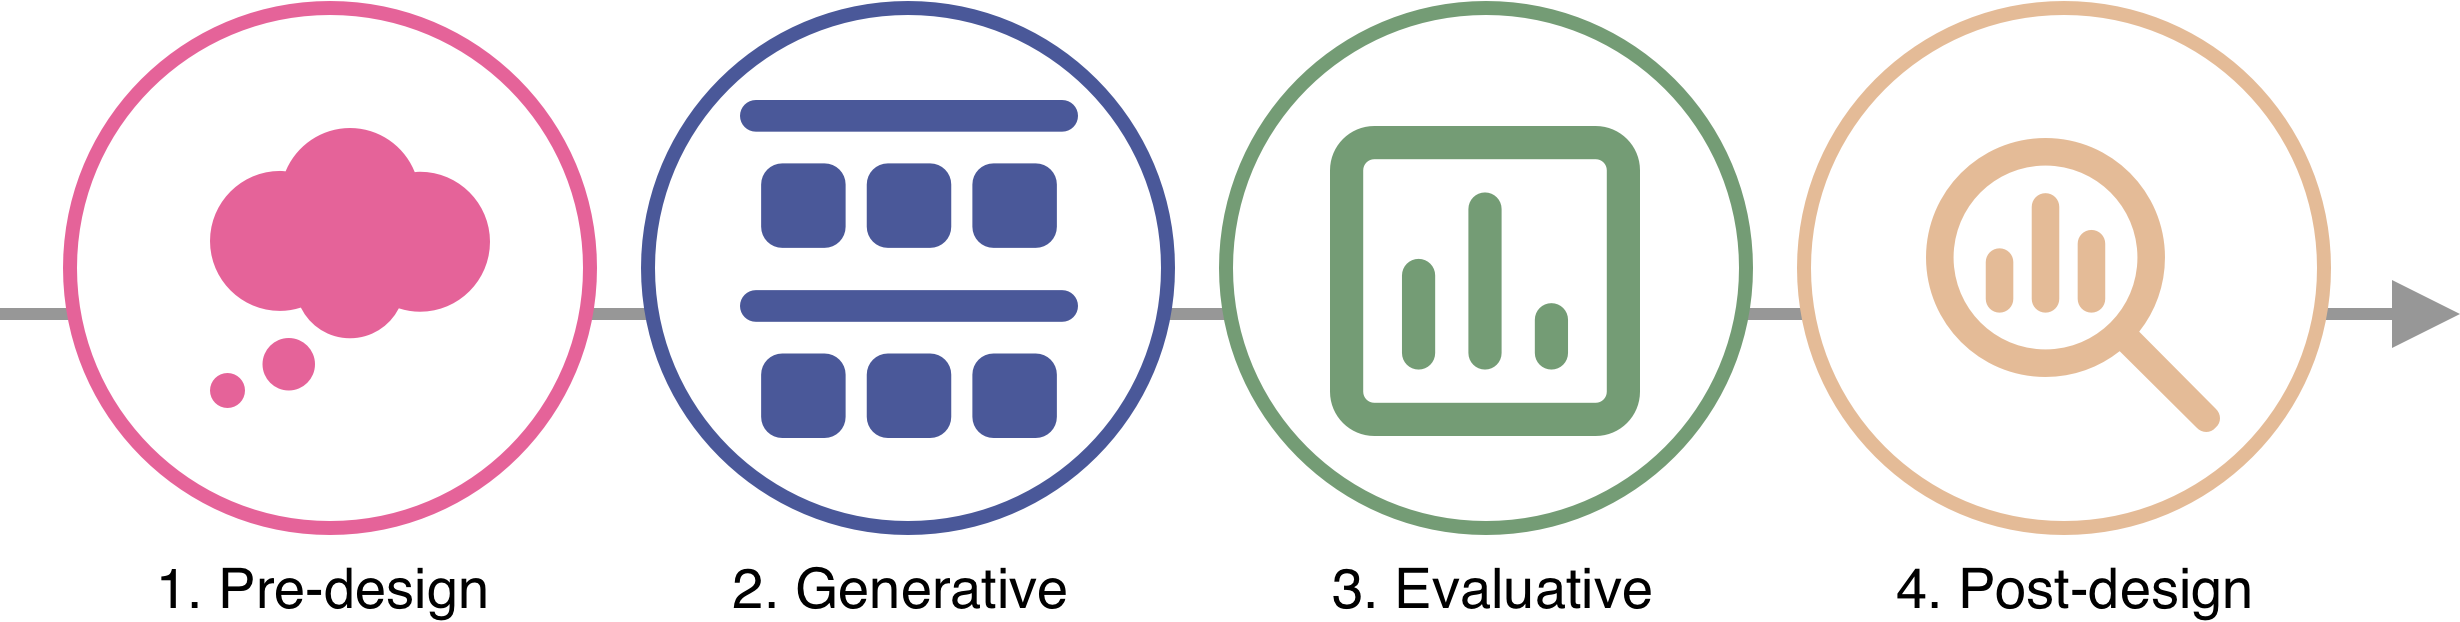
\includegraphics[width=0.8\linewidth]{Images/ChapterTwo/PhasesOfTech.png}
    \caption{Four phases of tech development \citep{suijkerbuijk_active_2019}}
    \label{fig:PhasesOfTech}
\end{figure}
In a recent systematic review of developing supportive technologies for and with people with dementia, \cite{suijkerbuijk_active_2019} categorise technology development into four phases: pre-design, generative, evaluative, and post-design (seen in fig \ref{fig:PhasesOfTech}). In this subsection, I dive into a series of dementia-HCI studies that involve people with dementia in the different stages of development. This sub-section aims to focus on the type of people with dementia who are included (or instead excluded), alongside the type of methods and approaches researchers adopt to involve the voices of people with dementia.

\subsubsection{Pre-design}
\label{BL:Pre-Design}
This literature review began by outlining the different ways HCI researchers have adapted participatory approaches to involve and represent people with dementia in the different phases of technology development. 

\section{Drawing from work outside dementia-HCI space}
\label{BL:Outside-HCI}
From the HCI literature, I have highlighted the different ways researchers have adapted and adopted participatory approaches to better suit the needs of their participants through the various technology phases. Through reviewing this literature, they are three particular areas of interest that require further consideration:
\begin{itemize}
    \item The majority of HCI work has focused on mild to moderate stages of dementia for participation. Further, HCI literature also targets the individuality of the person with dementia. While this is critical for building dementia technology, it has overlooked alternative stakeholders such as care partners, residency staff, and those involved in designing technology. This has resulted in an unrepresentative perspective of designing for involvement with people with dementia. 
    
    \item The ethical consideration needed to include the voices of people living with dementia in HCI research has resulted in a strong relational basis for design practice. However, dementia in HCI is still somewhat new, and dementia-HCI could benefit from understanding the type of ethical complexities non-HCI dementia and care practices have encountered.
    
    \item In recent dementia-HCI literature, researchers have examined how dementia advocates use technology to tackle stigma and dementia awareness. Exploring alternative ways researchers and people with dementia tackle stigma will provide insights into the potential ways to support dialogue between people with dementia and other stakeholders who may lack dementia experience.
\end{itemize}

\subsection{Co-design vs co-creation in advanced dementia}
Involving people with advanced dementia in research adds additional complexities because participants cannot contribute verbally to the research. However, similar to the work in HCI by \cite{lazar_using_2014} and \cite{foley_student_2020}, dementia researchers outside the space of HCI have also relied on creative and visual approaches to meaningfully engage and include people with advanced dementia in the research process.

In \cite{tsekleves2020engaging} playful practice for engaging with advanced dementia, they report on the blurry nature of their approach being co-design or, more accurately, known as co-creation. As \cite{sanders2008co} describe, co-creation orients collective creativity where the designer/researcher forms ideas from the user's needs, daily life and abilities. At the same time, \textit{"Co-designing threatens the existing power structures by requiring that control be relinquished and given to potential customers, consumers or end-users."}

In working with the four-stage design process (that I described in \ref{fig:PhasesOfTech}), \cite{tsekleves2020engaging} highlights that while people with advanced dementia could contribute to the generative and evaluative design stages, carers, researchers and support workers were required to contribute to the project. People with dementia's contribution to the generative and evaluative stages were accessible because the co-creative activities were in the moment, providing the team with thoughts and interactions during the session. Similarly, \cite{treadaway_sensor_2016} report on playful activities involving and engaging people with dementia in the development of sensory e-textiles. They co-created several sensory textiles by involving technical experts, care providers, and people with dementia in various stages of the design process. While people with dementia were not involved in the pre-design phase, they were part of the evaluative stage which the authors describe as the 'make together' process by exploring how the prototypes provide comfort, soothing and ways to facilitate in the moment interactions between the person with dementia and family members.

Returning to \cite{tsekleves2020engaging}, given the nature of cognitive and memory deficits when working with dementia, the authors argue that building truly co-design relationships with people with dementia is rarely achievable. Given the ethical challenges of co-design that I described previously and the complexities researchers might face in building continuing relationships with participants due to their progression of dementia, it is particularly timely to begin to unpack the collaborative nature of co-design and co-creation to understand the priorities for people with dementia in the design process. Therefore, researchers must explore to what extent should the research team contribute input into the design process versus the support they provide participants to contribute their input into the co-design process.

% Might want to build up this section by talking about the valuable nature of involving the interests of others.


\subsubsection{visual methods for inclusion}
When working with people in the later stages of dementia, traditional research approaches such as interviews and focus groups may be challenging for those who are non-verbal \citep{swarbrick2015quest}. Alternatively, researchers have studied the everyday interactions of people with dementia through an ethnographic approach \citep{kontos_ethnographic_2004,morrissey_value_2017,foley_care_2019}. Generally, ethnographic data collection consists of observational and field notes that multiple dementia-HCI researchers have adopted; however, more visual data collection processes have yet to become common in the dementia-HCI area. One visual data collection process that a small number of social researchers in dementia have started to use is videography \citep{phillipson2018more}.

\cite{campbell2017video} explored ways visual methods would enable the researchers to understand the interactions and experiences of a care-based hair salon focusing on the interactions between people with dementia and care staff. The authors captured 48 hours of video and more than 300 hours of unstructured observations through the extensive ten-month study. The authors highlight the practicability of using film to analyse and involve advanced stages of dementia. For instance, one participant, Audrey, who has advanced dementia, expressed her enjoyment or frustrations during her haircut through varying sounds and how she positioned her body or looked directly at herself in the mirror. In these instances, the video captured the ways Audbrey interacts and communicates with the world through her body. 

Additionally, while Campbell and Ward describe film may contribute to the controlling of what is and is not filmed, the authors emphasise that film can be empowering for some participants by choosing where the camera may go; letting people with dementia lead the interactions; and the researcher being asked questions about the process as they integrate themselves into the care-home. 

Similarly, \cite{cook2002using}, who uses video observation in dementia, describes how the physical object of the camera moves the conducting of research to more of an 'event', where participants are aware of being filmed and can take control of being involved resulting in an ongoing process of consent. In contrast, Cook states that her participants would rarely know what she was doing when taking field notes where she would fade into the room's background. Cook also describes how participants could easily ask to stop the filming by either leaving the room or asking Cook. While the awareness of the camera may complicate how natural the everyday interactions are, the physical object of the camera provides a sense of visibility and transparency to participants where they can be aware of what is being captured and filmed. Finally, it is worth noting how people with dementia may be represented in the film. In Campbell and Ward's work, they highlight a series of sensitivities required to ensure film does not misrepresent the participants. Similar to other data collection processes, film cannot describe the whole story, which may mean it could be interpreted differently and understood by different viewers. While researchers must be aware of who they share the data with, considering how participants might own their data could provide opportunities for understanding how they represent themselves and who they want to share their stories with.

With this in mind, visual data collection processes such as video provide people with dementia many opportunities to be involved through capturing 'moments' that are not reliant on verbal language and reflecting on history or personal experiences. Furthermore, \cite{majlesi2017video} reports how video collection might reveal interactions between couples where one person has dementia. Their study observes that while the care partner leads the conversation and speaks on behalf of the person with dementia, the video data analysis supports the person with dementia in a co-tellership role by observing their non-verbal interactions with the conversation.


\subsection{Ethical dilemmas in dementia}
\label{BL:EthicalDilemmas}
In this literature, I have described that the inclusion of people with dementia is the best practice and is the dominant view in researching such topics. However, as highlighted in the HCI literature, involving people with dementia presents complex ethical and methodological issues that require a more sophisticated examination. Keeping in mind that I have discussed HCI ethical challenges such as developing rapport; building researcher-participant relationships, technical longevity issues; and time investment, this section unpack issues regarding consent, gatekeepers, and managing power dynamics.

\subsubsection{Consent}
The process of participation for people with dementia can stumble on issues at the first hurdle - consent. Despite involving people with dementia being regarded as best practice, researchers are often challenged by ethical approval from institutional ethical review boards that define ethical practices through institutional ethical procedures. In the UK, these bodies are known as 'Ethical Review Boards' (ERBs) that are present across all universities and are put in place to ensure research follows sound ethical principles and puts the welfare of participants at the forefront of the research \citep{pachana_can_2014}. While most, if not all, often reflect the philosophical basis of morality, ERBs are significantly shaped by their culture and society, resulting in a vastly different set of expertise and approaches to reviewing research ethics \citep{flicker_ethical_2007}.

While these ethical guidelines set a course for research that seeks to ensure that both the participant and research institute are informed and protected, many prominent interdisciplinary research approaches, such as participatory design and qualitative, can be considered ethically questionable ERBs. \cite{bell_censorship_2014} argues that many ERBs' approaches to ethics align more with biomedical and experimental scientific methods, which fail to reflect the multiple ways of generating knowledge that encompass the third wave of HCI \citep{bodker_when_2006,lazar_critical_2017}. \cite{carla_introducing_2013} suggests that for qualitative researchers,\textit{"ethical issues arise from the very beginning of the research, they stay with us throughout our interactions with our research participants, and they continue to be relevant throughout the process of dissemination of the research findings"}, and call for a prolonged and adaptable approach to ethical research design. 

For most research, these guidelines may be relatively straightforward. However, people with dementia might become excluded from research as ERBs may see the involvement as too high risk or informed consent is inappropriate. \citep{dewing2004including}. They are several person-centred consents processes that emphasise consent to run through the entirety of the research. For instance, \cite{dewing_participatory_2007} describes the process consent method as an ongoing process between the researcher and the participant. This method moves away from the 'one-off' act of attaining consent that is flawed for people with dementia, where the decision on the day of consent may not reflect their choice the following day. However, while researchers are acknowledging alternative approaches for consent, ERBs may be of a different mind and hesitant to consider alternatives to more traditional approaches to consent.

\subsubsection{Gatekeepers}
Beyond the institutional gatekeeping role of ERBs, researchers must consider the gatekeeping roles defined by family members, care partners, care staff, and clinicians who may help or hinder the inclusion of the person with dementia \cite{ries2020ethical}. On the one hand, gatekeepers might refuse people with dementia to participate; stress their interests over the person with dementia; decide on behalf of the researcher and people with dementia on who should be involved; and influence access to participants. On the other hand, gatekeepers can provide support to the person with dementia through research activities; provide valuable information about the person with dementia's history, desires and needs; and share their strategies with the researcher to adapt their participatory approaches \citep{novek2019safe}.

While recognising the challenges of involving gatekeepers is important, \cite{grill2014facilitating} work on study partners in clinical trials demonstrates that people with dementia are less likely to participate in research without a care partner or the support of staff/volunteers from a care home or local dementia group. With this in mind, building a relationship with the person with dementia, and the 'study partner' is essential to ensure the willingness and interests align to participate in the study. \cite{bartlett2019strategies} highlight how getting to know gatekeepers, provides insight into what strategies they might use for recruiting and consenting. For instance, the author describes one of her PhD students spending time with a medical photography team at the hospital to gain initial feedback on her idea and develop a tailored plan for recruiting and consent for her participants. 

Additionally, \cite{thoft2021journey} describes gatekeepers pushing their agenda where they were told not to include spouses, as they had taken over the conversation in previous research, meaning the person with dementia was overlooked. The author explains further that they had to manage spouses through sharing project information to ensure they felt included while also centring the person with dementia in the research. From these examples, it is apparent that researchers need to get the balance right between stakeholder needs (people with dementia, gatekeeper, care partners) and the requirements of the original study design. As such, similar to working with people with dementia, ensuring gatekeepers are satisfied takes time to build relationships and sensitivity is required to respect the individual needs and expectations of the gatekeepers.

\subsection{Public perception of dementia}
\label{BL:PublicPerception}
As highlighted in this literature review, one of the more prominent challenges people with dementia face is how stigma defines their interactions and experiences with dementia. While the literature describes that terms like 'demented' and 'sufferer' negatively contribute to the way people see dementia, many people with dementia will self-stigmatise, which urges people with dementia to isolate themselves from social interactions and hide their illness from others \citep{milne2010d}. There has been a growing interest in looking at what can be done to challenge stigma and discrimination in dementia in recent years. For instance, policymaking has a pivotal role in forming dementia strategies to "address stigma and raise public awareness about dementia" to present a positive image of dementia and challenge negative attitudes in public opinion. 

Researchers are improving this area of work by maximising their impact outside of academia by using research to \textit{"facilitate societal, economic, political or legislative change"}. \cite{tischler2020using}, who explored public engagement activities to challenge harmful ideas of dementia, argue that research must embed itself in practice to ensure academic knowledge is communicated outside of venues and academic journals. For example, \cite{kontos_raising_2018} uses theatre to demonstrate the changes in relationships and struggles that a diagnosis of dementia presents. The theatre play, Cracked, follow a person with dementia and their family on a journey to see beyond the diagnosis. Throughout the play, the director creates an immersive space for the audience to question and reflect on their assumptions, sharing and refining a more sensitive, nuanced narrative of dementia. Through seeing a dementia discourse that has been popularised by its authors, the watching of the play intends to inspire the public to see dementia in alternative ways, the importance of ethical care, and how people with dementia can maintain strong relationships \citep{gray2020knowledge}.

This recent work resonates with the ongoing drive toward alternative creative approaches for public health and cultural awareness to elucidate conversations and question assumptions. \cite{carter2021effectiveness} invited people with dementia to share their experiences to identify a set of themes that an educational game could tackle. As a result, the authors developed a digital game, \href{https://www.dementiagame.com}{dementiagame.com}, where the public answers questions that challenge misconceptions, i.e. \textit{"True/false - you should only spend time with a person with dementia if you are trained"}. From the results, the authors report the public gaining significant improvement in their attitude toward dementia. However, the authors argue that while this may be beneficial to upskill the public on dementia assumptions, \textit{"strategies that facilitate great social inclusion"} must be recognised as a priority to deescalate stigma and misconceptions about dementia. Therefore, how the public may engage with such sensitive topics should be explored and vice versa - how do people with dementia share their experiences and why?

people with dementia's motivation to share their experiences of living with dementia seems to be twofold: writing allows a reclamation of social identity through sharing their thoughts and feelings, and second, sharing their experiences helps not only family members, but also the public to look past the diagnosis of dementia by demonstrating life continues to be rich and meaningful post-diagnosis \citep{ryan_dementia_2009}. Sharing lived experiences can also be seen in the recent proliferation of blogs, presentations, and personal books advocating for changes in media and public portrayals of dementia, which might counteract dominant misconceptions about, and stereotypes of, the condition \citep{christine_bryden_dancing_2005,bryden_challenging_2020}. While this creates an opportunity for public engagement, the extent to which the 'public' engages with these narratives is underexamined, begging the question: how can these experiences be better positioned for societal change-making? Moreover, despite its benefits, such advocacy work is often associated with strain through the \textit{"psycho-emotional consequences of taking action" }\citep{bartlett_citizenship_2014} where advocates present themselves in an opposing dominant public view. For instance, Christine Bryden, a pioneering dementia advocate, will often show images of her brain scans in presentations to prove she has dementia as several advocates have been accused by medical practitioners of not \textit{"look[ing] or sound[ing] like [they] have dementia"} \citep{swaffer_but_2016}. In these instances, exploring ways to balance empathy and maintaining an individual's privacy and dignity is required.

With this in mind, including aspects of public engagement in design work with vulnerable groups such as people with dementia requires careful consideration. One challenge lies in how we engage with such complex (and often stigmatised) topics sensitively while encouraging public engagement, which in turn allows a greater extension of awareness and understanding around the topic of interest. For example, many expert researchers will have years of experience working with people with dementia, and are aware of both the importance of attuning to person-centred approaches \citep{fazio_fundamentals_2018} and language, but also of the damage negative and stereotypical ideas of dementia can have when used to emphasise a deficit or inaccurate image of life with dementia \citep{young_expanding_2019}. Moreover, \cite{niederdeppe2008message} highlight the formidable communication challenges faced when inviting a wider public to input on a sensitive topic due to unknown biases, priorities and cultural norms, which may risk having stereotypes aired publicly or even perpetuated. In response, the author's argue that different communication strategies may be required to educate and upskill the public on sensitive topics. Facilitating broader design engagement creates opportunities for collaborative learning between different communities to provide spaces for refining a more sensitive, nuanced public narrative of dementia, which may then be realised in the products, services, and systems we co-create \citep{costanza-chock_design_2020}. This may, in turn, shape the environments in which we learn about and support those living with dementia. Supporting collaboration and engagement in creating such artefacts through public-facing design events offers us one such opportunity. 

\section{Missing gaps in dementia-HCI literature}
\label{BL:Missing-gaps}
This literature review began by outlining how HCI researchers have adapted participatory approaches to involve and represent people with dementia in the different phases of technology development. This final section outlines four gaps of literature that explore the social and political structures that enable (or instead disable) those with dementia to participate and be recognised for their meaningful contributions. 

\begin{itemize}
    \item \textbf{Ethical practice in dementia-HCI}: At a time when the ethics surrounding technology design and deployment are receiving increased attention and given the current everyday ethical challenges described in this literature, there is a need for in-depth insights into understanding the ethical experiences and practices in the field of dementia-HCI.
    
    \item \textbf{Representation of technology and dementia through public engagement}: As dementia advocates share their lived experiences to counteract dominant misconceptions about the condition, the extent to which the 'public' engage with these narratives is underexamined. For that reason, HCI literature might consider a) how technology contributes to people with dementia sharing their experiences online, and b) how might public engagement events support the learning and collaboration around dementia and technology.

    \item \textbf{Promoting learning around dementia and technology}: In the first section of literature on the different phases of technology development in dementia, I highlighted the extensive involvement of different skill sets and stakeholders who are part of the design process. While working closely with people with dementia is a priority in designing meaningful technology, designers, developers and researchers might require collaborative and learning tools to support design research, creativity, and technological development and implementation.  
    
    \item \textbf{Attending to mutual collaborative relationships}: Traditionally, studies often separate care partners and people with dementia with the expectation that they require different needs from one another. While perhaps that might be true in some cases, the literature highlights that when spending time with the ecology of care, the overall design includes a variety of interests and interactions that the ecology of care desires. With this in mind, designing with people with dementia should also target care partners, family and friends to be part of the design processes and be meaningfully represented in the technology we create.

\end{itemize}

\subsection{Ethical practice in dementia-HCI}
\label{BL:gap:Ethics}
Participatory and co-design projects have innovated methodological approaches to design, which are necessary to support people with dementia to engage meaningfully in the co-design process. The literature illustrates ways to engage in longer-term projects, work with the family ecology of care, and navigate gate-keeping within institutions. This includes: treating the person with dementia as an individual in context; including the person with dementia in research processes that are explicitly aiming to improve their quality of life; acknowledging that dementia is a complex experience that often also includes social complexity \citep{keyes2019living}, ageing and multi-morbidities \citep{buse_materialising_2016}, which require attuning to in design and research responses. It can be argued that these design decisions offer particular ethical stances that appear essential to both the success of HCI projects in this context and ensure the researcher-participant relationship is navigated with mutual respect and care \citep{foley_care_2019}. However, in contrast to the breadth of literature outside of HCI that reflects and demonstrates the relational complexities seen in the everyday interactions of working with people with dementia, dementia-HCI has yet to make these ethical processes more visible.

While dementia-HCI researchers can learn a lot from non-HCI literature on dementia, introducing technology brings additional complexities concerning privacy and data storage; health and educational support; technology longevity, and technology responsibility \citep{cornejo_vulnerability_2016}. Additionally, gatekeeping and consent issues described in the literature need further consideration regarding the influence of ERBs that uphold our work. \cite{pachana_can_2014} further highlight that committees may be \textit{"subject to the same biases and stereotypes present in the general population"}. ERBs unaware of such biases may focus on the aims of protection instead of the approval of research that attends to topics such as agency and ensures meaningful participation. Further complexity arises since ERB decisions vary even within the same country or region \citep{edwards_research_2004}. This is because the decisions and reasoning's are made at a university level and influenced by cultural and local norms and customs. Thus, the disciplinary changes in working with populations such as dementia are not necessarily matched at the level of those who make decisions about what research is and is not allowed when carrying out participatory work with participants who are considered 'vulnerable'.

These challenges have been navigated and discussed in detail through ACM Town Halls and conference workshops \cite{frauenberger_research_2017, munteanu_sigchi_2019}. Researchers have been invited to reflect and consider the ethical challenges they face within this space. While recent work in HCI has begun to examine the role of ethics in HCI research - particularly studies that work within sensitive settings, there is a need to come together as a community of practice to identify institutional and relational ethical challenges. In light of this, examining the ethical complexities faced in dementia-HCI work might provide valuable insights into ways to ensure meaningful and engaged research with marginalised groups is central to the design of technologies and systems.

\subsection{Representation of technology and dementia through public engagement}
\label{BL:gap:engagement}
Over the years, people with dementia have shown a growing interest in raising general public awareness about dementia by participating in panels, workshops, blogs and presentations. \cite{innes2021s} interviewed six people with dementia who are part of a Dementia Associate Panel (DAP), highlighting how empowering and affirming people with dementia felt when facilitating and educating people on dementia. The study participants continue to describe the benefits of such involvement in public awareness as it promotes a broader perspective of dementia and improvements in dementia support and services.

Within HCI, design and development domains, hackathons have become a popular approach for researchers and organisations to bring together the public to develop new paths to research, ideate, and test software or products. Typically, hackathons have been organised and sponsored by businesses or universities to allow undergraduates to gain experience and practice new skills and potentially build connections between the attendee and organisation recruiters or employees. Hackathons are often coupled with rewards and prize money for the winning team as an enticement to spend time building a demo and/or presentation \citep{johnson_civic_2014}. Hackathons have also been adopted as opportunities for co-operative makerspaces focusing on health and other community-based issues: for example, hackathons for women’s health \citep{paganini_engaging_2020}, and self-harm \citep{birbeck_self_2017} have offered key insights into how interdisciplinary teams can come together to shape innovative technical responses to complex topics and wicked problems. 

One challenge lies in how we engage such sensitive topics in HCI while encouraging public engagement and facilitating opportunities for collaborative learning and awareness around the topic of interest. While it takes time for researchers to become aware of the sensitivities required for working with such a population, hackathon formats expect the same sensitivities to develop quickly – usually at the weekend. Therefore, it is not surprising that prior work has indicated that some design outputs may be unsuitable or feed into stigmatising ideas of the group or topic at the centre of the design event \citep{toros_co-creation_2020}. Prior work has considered ways to sensitise attendees on the event's topic through presentations, workshops \citep{hope_hackathons_2019}, and inspiration packs \citep{birbeck_self_2017} to upskill participants who may hold outdated or stereotypical attitudes. Given the potential challenges of such public design events, it might be worth considering how representation and attitudes on dementia may be presented in more technical public design events. Further, with people with dementia engaging in public awareness through sharing experiences, facilitation, and presentations, how might design events be structured to support these sensitive conversations better.


\subsection{Promoting learning around dementia and technology}
\label{BL:gap:Learning}
As described in the literature, to support to help foster empathy with, and understanding of, a person with dementia's experience, there has been a push from dementia activists toward using online interactions and bespoke forums and Twitter to raise awareness and further challenge the stigma surrounding dementia \citep{talbot_how_2020}. Likewise, \cite{lazar_safe_2019} work on dementia activism shares insights into people with dementia proactively coming together online to raise awareness and challenge stereotypes and stigma of current portrayals of living with dementia. This work highlights the online work of a committed group of people with dementia, curating and publishing their experiences, personal views, and providing opportunities for dialogical interactions to happen. However, understanding how those making design decisions on behalf of people with dementia remains sparse. 

Much research in HCI has been devoted to the development of toolkits and other creativity support mechanisms, which have variously been used to support design research, creativity, and technological development and implementation \citep{broderick2020theory}. \cite{ledo2018evaluation} write that toolkits within HCI provide: a) simplifying and fast-track creation, b) assistance in problem-solving processes, c) help to engage new audiences d) help to adapt tools within users workflows and e) support replication to enable scaling. \cite{peters2020toolkits} suggest tools be more \textit{"consciously culturally-tailored" \citep[pg.20]{peters2020toolkits}}. This may require involving audiences in the creation and customisation of the tool. Similarly attending to the practical use of such kits, in a recent review of open-source fairness toolkits, \cite{lee2021landscape} raise a valuable concern, stating creators of such toolkits should \textit{“remain vigilant to ensure their adoption is aligned to the over-arching goal: to ensure our algorithms reflect our ethical values of non-discrimination of fairness” \citep[pg.12]{lee2021landscape}}. In cases like these, the provision of tools that may be freely used and reshaped by a user community requires further thought about the roles of moderation or expertise, particularly when toolkits may be intended for use or application in marginalised settings. This open-source framing also, interestingly, opens up the possibility that toolkits might move from being static resources (even so far as being printed, boxed and shipped), to being something that evolves and develops over time (a fluid and unfinalisable design tool).

In reviewing the above, we see that many of toolkits have been developed in response to a given problem or design challenge - whether that has been engagement with a particular community, or to provide insight and knowledge on a complex or novel topic. Prior work has highlighted that the content of such toolkits requires careful consideration, and often a set of expert curators to ensure content is ethical and sensitively designed. However, returning to our dementia literature, such work involving people with dementia requires adaptability to ensure inclusive and meaningful engagement. Furthermore, while there are many different types of toolkits that we look to for inspiration for applications within dementia, we must ensure that the toolkits will adapt and fit into the user’s workflow. In turn, this raises the question of what sorts of toolkit interactions we should provide to designers and developers that allow them to design with people with dementia collaboratively.


\subsection{Attending to mutual collaborative relationships}
\label{BL:gap:relationships}
Fostering independence is central in person-centred approaches, where the person's individuality and abilities are valued. \cite{leverton2021supporting} describe how homecare workers use the person with dementia's identity, wishes, and extensive knowledge about the person to support independence by offering meaningful choices and involvement in decision-making. The independency for making decisions is an integral aspect of citizenship - one that has been examined within disability research and within dementia \citep{meissner_-it-yourself_2017,samsi_everyday_2013}. However, as dementia is a progressive condition, the change and decline pose challenges to the person with dementia's ability to make decisions. While it is not uncommon for a partner to take it upon themselves to assist or take over the individual's roles within the family, several vital decisions must be carefully considered, such as care planning, care-home placement and eventually - end of life \citep{fetherstonhaugh_decision-making_2017}.

\cite{fetherstonhaugh2013being} highlight the importance for people with dementia to be involved in decisions that require the care partner to learn how to enable those decision-making processes best. For instance, one participant describes "maintaining close family relationships and trusting friendships" as a way to feel central to the decisions through being acknowledged and consulted. The findings illustrate this as essential in even the minor day-to-day interactions such as taking the bins out, choices for dinner, and day-out activities. Attending to more interdependent and support strategies requires careful consideration towards care partners, knowing the balance between subtle support versus taking over.

Moreover, despite the benefits of supporting the decision-making processes, this can cause a burden for both parties. This is further complicated when the literature demonstrates the need for people with dementia to shared their lived experiences and push for societal change. \citep{johnson_older_2019} draw attention to the strain and potential 'burdening' that this can cause, as people with dementia already often feel as though they need to support others living with the condition and actively challenge misconceptions and stereotypes that the public may hold. This raises interesting challenges about how to ethically engage this community in design processes without overburdening their participation. With this in mind, HCI research needs to examine the ways participation and technology may support the involvement of different voices from the ecology of care while ensuring the person with dementia is well represented and involved in the design making process. 

\section{Summary}
\label{BL:summary}
This review has detailed dementia literature regarding how we represent the experiences of people with dementia and involve them in participatory work. The literature review started with a discussion on the ongoing shift from a bio-medical approach to a more person-centred approach that has been adapted and adopted by the HCI community. Through this discussion, I have highlighted the breadth of work done in HCI that emphasises the need for relationship building, working within ecologies of care, and engaging with participants' creativity. From here, I broaden the literature review to consider dementia literature outside the HCI space. This section examines various ethical considerations for including later stages of dementia, consent and navigating gatekeeping within institutions and organisations. Additionally, to explore the missing gaps in dementia-HCI, I introduce literature concerning the public perception of dementia that describes how HCI work might benefit from such public-facing engagement to support the collaboration of designing technology with people with dementia.

The final section outlines four avenues of investigation for this thesis that orients toward a more critical perspective of dementia. These avenues are not intended to be exhaustive but rather to move towards a multidimensional understanding of dementia and question the adapting roles and situations people with dementia may have within their relationships. To conclude this chapter, it is worthwhile to revisit the research questions in retrospect to the missing gaps found in the literature review:


% Please add the following required packages to your document preamble:
% \usepackage[normalem]{ulem}
% \useunder{\uline}{\ul}{}
\begin{table*}[htp]
\caption{Research questions in regards to the background literature}
\label{BL:RQ}
\begin{tabularx}{\textwidth}{@{} Y|Y @{}}
\textbf{Research question} & \textbf{Areas to explore from literature review}  \\ \hline
How can we use participatory design approaches to provide meaningful and engaging experiences for people with dementia? & Participatory approaches must be co-created with people with dementia and their care partners to improve engagement and inclusion.  \\ \hline
What are the ethical implications for people with dementia to participate in HCI research? & Outside HCI, dementia researchers have built a breadth of information on the ethical complexities of working and representing people with dementia. While the literature review highlights a handful of dementia-HCI papers that reflect on the ethical challenges, there is a gap in the literature to understand the complexities from an HCI perspective.
  \\ \hline
What are the competing interests and expectations to support meaningful dialogue in dementia design research when involving multiple stakeholders - such as people with dementia, developers, designers and researchers? & Lack of involvement of stakeholders who are part of the design process  \\ \hline
\end{tabularx}
\end{table*}


In the next chapter, I describe the methodologies used for this research which examines the role of participatory design approaches to understand the relationships between people with dementia and diverse stakeholders.
